\documentclass[]{beamer}
\usepackage{tikz}
\usepackage{listings}

\usetikzlibrary{shapes.geometric, arrows}

%% The style for the flow chart
\tikzstyle{process} = [rectangle, text width=3cm, minimum height=1cm, text centered, draw=black, fill=orange!30]
\tikzstyle{arrow} = [thick,->,>=stealth]


\begin{document}
  \begin{frame}{Statistical analysis value chain}
    \begin{center}
      \begin{figure}
        \centering
        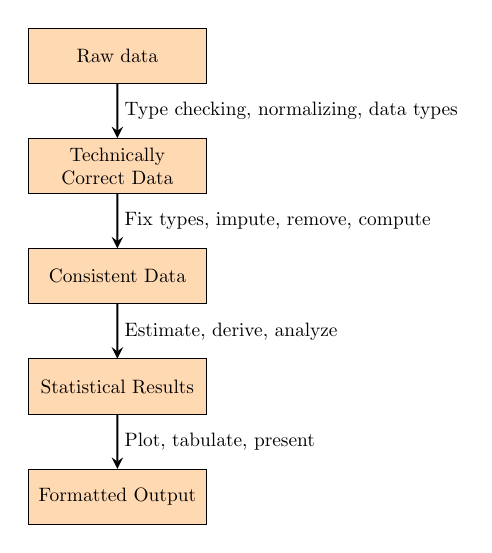
\begin{tikzpicture}[scale=0.7,  transform shape, node distance=2cm]
          \node (raw)  [process]                {Raw data}; %
          \node (tech) [process, below of=raw]  {Technically Correct Data}; %
          \node (cons) [process, below of=tech] {Consistent Data};  %
          \node (stat) [process, below of=cons] {Statistical Results}; %
          \node (form) [process, below of=stat] {Formatted  Output}; %
          
          %% Connections
          \draw [arrow] (raw)  -- node[anchor=west] {Type checking, normalizing, data types}   (tech); %
          \draw [arrow] (tech) -- node[anchor=west] {Fix types, impute, remove, compute}       (cons); %
          \draw [arrow] (cons) -- node[anchor=west] {Estimate, derive, analyze}                (stat); %
          \draw [arrow] (stat) -- node[anchor=west] {Plot, tabulate, present}                  (form); %
        \end{tikzpicture}
        \caption{Statistical analysis value chain (adapted from \cite{})}
      \end{figure}
    \end{center}
  \end{frame}


  \begin{frame}
    \frametitle{Raw data}
    
    Raw data can be any source of information that can be processed in
    a computing device represented in any format. Examples of raw data include:
    
    \begin{itemize}
    \item Text documents
    \item Chemical compounds (perhaps represented as graphs)
    \item Usage data (e.g., log files)
    \item Images
    \item Speech
    \end{itemize}
  \end{frame}

  \begin{frame}[containsverbatim]{Loading Raw data in R}

    In this tutorial we will assume that data is given in a
    ``rectangular format'' where each row depicts an object of
    interest (a document, a chemical compound or an image) and the
    columns denote a particular feature.
    
    
    \begin{lstlisting}[language=R]
      read.table()
    \end{lstlisting}
  \end{frame}

\end{document}
%%% Local Variables:
%%% mode: latex
%%% TeX-master: t
%%% End:
